%chapter 2
\chapter{A Probabilistic Graphic Model for Grasping Problem}
\label{chapter2}
\section{Introduction}
As we mentioned in the previous chapter, the essence of the robotic grasping problem is to control the actuators to achieve grasping success. Due to the process uncertainty, the same measurement and the same actuator control may not result in the same outcome.  A lot of uncertain factors are involved in the grasping process. These include imperfect sensor input, the shape of an object, precision of control and satisfaction of task constraints.  These include sensor measurement, shape of object, precision of control and satisfaction of task constraints. They are all influence factors contributing to a grasp success. Therefore, it is more reasonable to use a probabilistic model to estimate the probability of grasp success rather than using a deterministic model. As the success probability of grasping depends on many factors, direct modeling the problem from the factors to success probability is complex and hard. One way to handle the complexity is to model the grasping problem using probabilistic graphic models~\cite{Koller1989}.  

Probabilistic graphic models use a graph structure to represent a probabilistic distribution over high dimensional space. The major advantage of using a graph-based representation is one can break the modeling of complex probability distribution over every possible variable into simple small factors. The joint distribution of every possible variable is simply the multiplication of these small factors. Specifically,  we can break up the modeling of joint distribution over all the factors which may influence the success into smaller manageable probability models.  We use one family of the probabilistic graphic models called `Bayesian Networks' to model the grasping problem. The `Bayesian Networks' uses a directed graph to represent    the probability distribution. A directed graph is composed of a set of nodes and directed edges. The nodes specify random variables that represent influence factors. The edges define the direction of dependency between factors. The reader can refer to~\cite{Korb2003} for a more formal description of  `Bayesian Networks.'  


\section{Probabilistic modeling of grasping using Bayesian networks}
In this section, we introduce a general description for grasping problems using a Bayesian network. We first define a set of variables for the problem. A graph is then proposed to model the dependency between the variables. Then we explain that solving grasping problems is equivalent to solving inference tasks under the condition that a subset of the defined variables is observed.   
\subsection{Variable definition and graph structure}
The first variable that we define for the grasping problem is the outcome of a grasping process $S$. The outcome is a discrete random variable which takes two values to specify whether a grasping process succeeds or not. One standard definition of the success is whether the gripper of a robot achieves force closure on the object. However, this definition only considers the result of grasp acquisition itself. As grasping of an object may also have a purpose, the task intention of a grasp should also be considered as a part of grasp success. Therefore, we define the success of a grasping process not only based on force closure property but also on whether the task constraint is fulfilled. Thus, we define another two discrete variables $F$ for whether the gripper achieves force closure condition and $C$ for whether constraints defined by the grasping task is fulfilled. Consequently, the outcome of a grasping process $S$ only depends on $F$ and $C$. Now let's consider which factors can influence the force closure condition $F$. It is reasonable to think that object state $X$ and robot controls $U$ jointly affect the force closure condition. As the object state $X$ is normally not observable and derived from the sensor measurement, we define $Z$ to be the sensor measurement that can influence the estimation of object state. The task constraint satisfaction $C$ represents whether a grasp configuration satisfies the condition regarding a specified task. Therefore, a task specification $T$ naturally influences the task constraint. Besides that without the grasp configuration, it is not possible to evaluate whether task constraint is fulfilled or not. Therefore, $C$ is also dependent on object state $X$ and robot control $U$.  

Based on the analysis of the factors and their dependencies we can model the  relationships of the factors into a Bayesian network. Figure.~\ref{fig:bnet} depicts the proposed network that we define for the grasping problem. All the variables surrounded by a box are binary-valued discrete variables, while the variables surrounded by an ellipse indicate their domain can be either discrete or continuous. All the defined variables are summed up in Tab.~\ref{tab:random_variable}.

\begin{figure}[!htbp]
\centering
%\def\svgwidth{0.6\linewidth}
%%% Creator: Inkscape inkscape 0.48.4, www.inkscape.org
%% PDF/EPS/PS + LaTeX output extension by Johan Engelen, 2010
%% Accompanies image file 'baysianmodel.pdf' (pdf, eps, ps)
%%
%% To include the image in your LaTeX document, write
%%   \input{<filename>.pdf_tex}
%%  instead of
%%   \includegraphics{<filename>.pdf}
%% To scale the image, write
%%   \def\svgwidth{<desired width>}
%%   \input{<filename>.pdf_tex}
%%  instead of
%%   \includegraphics[width=<desired width>]{<filename>.pdf}
%%
%% Images with a different path to the parent latex file can
%% be accessed with the `import' package (which may need to be
%% installed) using
%%   \usepackage{import}
%% in the preamble, and then including the image with
%%   \import{<path to file>}{<filename>.pdf_tex}
%% Alternatively, one can specify
%%   \graphicspath{{<path to file>/}}
%% 
%% For more information, please see info/svg-inkscape on CTAN:
%%   http://tug.ctan.org/tex-archive/info/svg-inkscape
%%
\begingroup%
  \makeatletter%
  \providecommand\color[2][]{%
    \errmessage{(Inkscape) Color is used for the text in Inkscape, but the package 'color.sty' is not loaded}%
    \renewcommand\color[2][]{}%
  }%
  \providecommand\transparent[1]{%
    \errmessage{(Inkscape) Transparency is used (non-zero) for the text in Inkscape, but the package 'transparent.sty' is not loaded}%
    \renewcommand\transparent[1]{}%
  }%
  \providecommand\rotatebox[2]{#2}%
  \ifx\svgwidth\undefined%
    \setlength{\unitlength}{266.48922058bp}%
    \ifx\svgscale\undefined%
      \relax%
    \else%
      \setlength{\unitlength}{\unitlength * \real{\svgscale}}%
    \fi%
  \else%
    \setlength{\unitlength}{\svgwidth}%
  \fi%
  \global\let\svgwidth\undefined%
  \global\let\svgscale\undefined%
  \makeatother%
  \begin{picture}(1,0.7093861)%
    \put(0,0){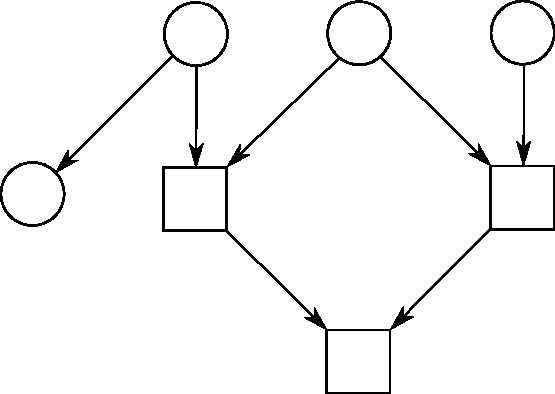
\includegraphics[width=\unitlength]{baysianmodel.pdf}}%
    \put(0.62968498,0.04171382){\color[rgb]{0,0,0}\makebox(0,0)[lb]{\smash{$S$}}}%
    \put(0.33638551,0.33553136){\color[rgb]{0,0,0}\makebox(0,0)[lb]{\smash{$F$}}}%
    \put(0.92239445,0.33553136){\color[rgb]{0,0,0}\makebox(0,0)[lb]{\smash{$C$}}}%
    \put(0.33586739,0.63038521){\color[rgb]{0,0,0}\makebox(0,0)[lb]{\smash{$X$}}}%
    \put(0.62968498,0.63149328){\color[rgb]{0,0,0}\makebox(0,0)[lb]{\smash{$U$}}}%
    \put(0.92671889,0.62934899){\color[rgb]{0,0,0}\makebox(0,0)[lb]{\smash{$T$}}}%
    \put(0.0420857,0.34096392){\color[rgb]{0,0,0}\makebox(0,0)[lb]{\smash{$Z$}}}%
  \end{picture}%
\endgroup%

%\resizebox{1\textwidth}{!}{%% Creator: Inkscape inkscape 0.48.4, www.inkscape.org
%% PDF/EPS/PS + LaTeX output extension by Johan Engelen, 2010
%% Accompanies image file 'graphicalModel_temporal.pdf' (pdf, eps, ps)
%%
%% To include the image in your LaTeX document, write
%%   \input{<filename>.pdf_tex}
%%  instead of
%%   \includegraphics{<filename>.pdf}
%% To scale the image, write
%%   \def\svgwidth{<desired width>}
%%   \input{<filename>.pdf_tex}
%%  instead of
%%   \includegraphics[width=<desired width>]{<filename>.pdf}
%%
%% Images with a different path to the parent latex file can
%% be accessed with the `import' package (which may need to be
%% installed) using
%%   \usepackage{import}
%% in the preamble, and then including the image with
%%   \import{<path to file>}{<filename>.pdf_tex}
%% Alternatively, one can specify
%%   \graphicspath{{<path to file>/}}
%% 
%% For more information, please see info/svg-inkscape on CTAN:
%%   http://tug.ctan.org/tex-archive/info/svg-inkscape
%%
\begingroup%
  \makeatletter%
  \providecommand\color[2][]{%
    \errmessage{(Inkscape) Color is used for the text in Inkscape, but the package 'color.sty' is not loaded}%
    \renewcommand\color[2][]{}%
  }%
  \providecommand\transparent[1]{%
    \errmessage{(Inkscape) Transparency is used (non-zero) for the text in Inkscape, but the package 'transparent.sty' is not loaded}%
    \renewcommand\transparent[1]{}%
  }%
  \providecommand\rotatebox[2]{#2}%
  \ifx\svgwidth\undefined%
    \setlength{\unitlength}{514.815004bp}%
    \ifx\svgscale\undefined%
      \relax%
    \else%
      \setlength{\unitlength}{\unitlength * \real{\svgscale}}%
    \fi%
  \else%
    \setlength{\unitlength}{\svgwidth}%
  \fi%
  \global\let\svgwidth\undefined%
  \global\let\svgscale\undefined%
  \makeatother%
  \begin{picture}(1,0.36762093)%
    \put(0,0){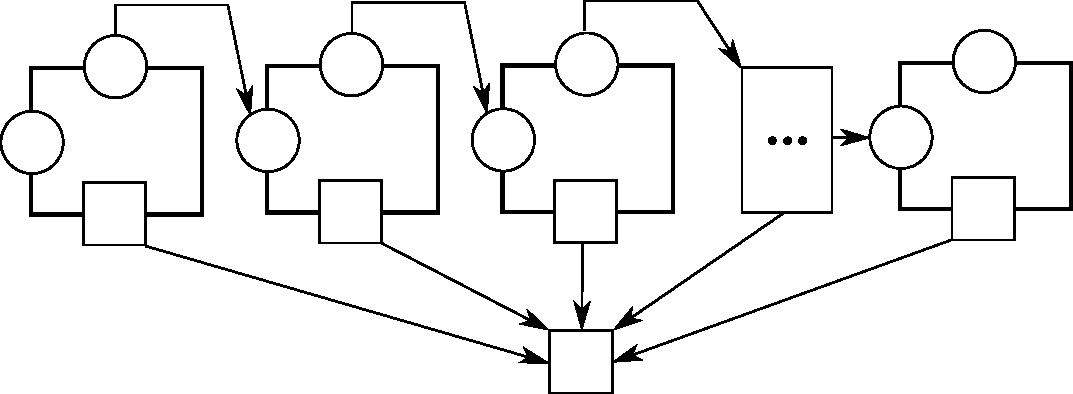
\includegraphics[width=\unitlength]{graphicalModel_temporal.pdf}}%
    \put(0.09547193,0.29665535){\color[rgb]{0,0,0}\makebox(0,0)[lb]{\smash{$U_0$}}}%
    \put(0.09407952,0.15956687){\color[rgb]{0,0,0}\makebox(0,0)[lb]{\smash{$S_0$}}}%
    \put(0.01881458,0.22563278){\color[rgb]{0,0,0}\makebox(0,0)[lb]{\smash{$Z_0$}}}%
    \put(0.31237857,0.29852096){\color[rgb]{0,0,0}\makebox(0,0)[lb]{\smash{$U_1$}}}%
    \put(0.31409408,0.16143247){\color[rgb]{0,0,0}\makebox(0,0)[lb]{\smash{$S_1$}}}%
    \put(0.23882916,0.22749837){\color[rgb]{0,0,0}\makebox(0,0)[lb]{\smash{$Z_1$}}}%
    \put(0.90558919,0.30139354){\color[rgb]{0,0,0}\makebox(0,0)[lb]{\smash{$U_n$}}}%
    \put(0.90419676,0.16430507){\color[rgb]{0,0,0}\makebox(0,0)[lb]{\smash{$S_n$}}}%
    \put(0.82893184,0.23037096){\color[rgb]{0,0,0}\makebox(0,0)[lb]{\smash{$Z_n$}}}%
    \put(0.53050271,0.02213156){\color[rgb]{0,0,0}\makebox(0,0)[lb]{\smash{$S_f$}}}%
    \put(0.53175169,0.29895161){\color[rgb]{0,0,0}\makebox(0,0)[lb]{\smash{$U_2$}}}%
    \put(0.53346717,0.16186314){\color[rgb]{0,0,0}\makebox(0,0)[lb]{\smash{$S_2$}}}%
    \put(0.4582022,0.22792902){\color[rgb]{0,0,0}\makebox(0,0)[lb]{\smash{$Z_2$}}}%
  \end{picture}%
\endgroup%
}
\resizebox{.5\textwidth}{!}{%% Creator: Inkscape inkscape 0.48.4, www.inkscape.org
%% PDF/EPS/PS + LaTeX output extension by Johan Engelen, 2010
%% Accompanies image file 'baysianmodel.pdf' (pdf, eps, ps)
%%
%% To include the image in your LaTeX document, write
%%   \input{<filename>.pdf_tex}
%%  instead of
%%   \includegraphics{<filename>.pdf}
%% To scale the image, write
%%   \def\svgwidth{<desired width>}
%%   \input{<filename>.pdf_tex}
%%  instead of
%%   \includegraphics[width=<desired width>]{<filename>.pdf}
%%
%% Images with a different path to the parent latex file can
%% be accessed with the `import' package (which may need to be
%% installed) using
%%   \usepackage{import}
%% in the preamble, and then including the image with
%%   \import{<path to file>}{<filename>.pdf_tex}
%% Alternatively, one can specify
%%   \graphicspath{{<path to file>/}}
%% 
%% For more information, please see info/svg-inkscape on CTAN:
%%   http://tug.ctan.org/tex-archive/info/svg-inkscape
%%
\begingroup%
  \makeatletter%
  \providecommand\color[2][]{%
    \errmessage{(Inkscape) Color is used for the text in Inkscape, but the package 'color.sty' is not loaded}%
    \renewcommand\color[2][]{}%
  }%
  \providecommand\transparent[1]{%
    \errmessage{(Inkscape) Transparency is used (non-zero) for the text in Inkscape, but the package 'transparent.sty' is not loaded}%
    \renewcommand\transparent[1]{}%
  }%
  \providecommand\rotatebox[2]{#2}%
  \ifx\svgwidth\undefined%
    \setlength{\unitlength}{266.48922058bp}%
    \ifx\svgscale\undefined%
      \relax%
    \else%
      \setlength{\unitlength}{\unitlength * \real{\svgscale}}%
    \fi%
  \else%
    \setlength{\unitlength}{\svgwidth}%
  \fi%
  \global\let\svgwidth\undefined%
  \global\let\svgscale\undefined%
  \makeatother%
  \begin{picture}(1,0.7093861)%
    \put(0,0){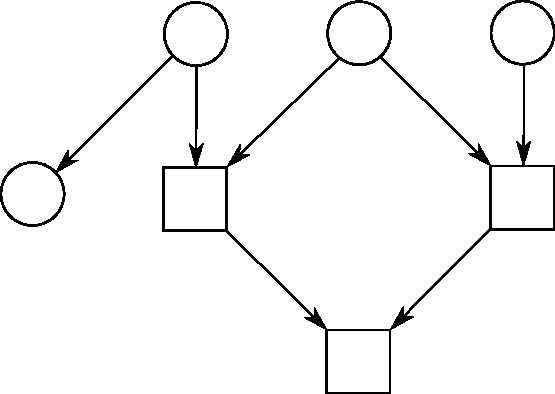
\includegraphics[width=\unitlength]{baysianmodel.pdf}}%
    \put(0.62968498,0.04171382){\color[rgb]{0,0,0}\makebox(0,0)[lb]{\smash{$S$}}}%
    \put(0.33638551,0.33553136){\color[rgb]{0,0,0}\makebox(0,0)[lb]{\smash{$F$}}}%
    \put(0.92239445,0.33553136){\color[rgb]{0,0,0}\makebox(0,0)[lb]{\smash{$C$}}}%
    \put(0.33586739,0.63038521){\color[rgb]{0,0,0}\makebox(0,0)[lb]{\smash{$X$}}}%
    \put(0.62968498,0.63149328){\color[rgb]{0,0,0}\makebox(0,0)[lb]{\smash{$U$}}}%
    \put(0.92671889,0.62934899){\color[rgb]{0,0,0}\makebox(0,0)[lb]{\smash{$T$}}}%
    \put(0.0420857,0.34096392){\color[rgb]{0,0,0}\makebox(0,0)[lb]{\smash{$Z$}}}%
  \end{picture}%
\endgroup%
}
\captionsetup{justification=raggedright}
\caption{A Bayesian network for the grasping problem. Variables surrounded by a box are binary-valued discrete random variables. Variables surrounded by an circle can be either continuous or discrete.}
\label{fig:bnet}
\end{figure}	

\begin{table}[!htbp]
\centering
\begin{tabular}{cl}
Variable & Description                              \\
$S$      & outcome of a grasping process            \\
$F$      & satisfaction of force closure condition \\
$U$      & robot control                            \\
$Z$      & sensor measurement                       \\
$X$      & object state                             \\
$T$      & task specification                       \\
$C$      & satisfaction of task constraints       
\end{tabular}
\caption{Definition of variables }
\label{tab:random_variable}
\end{table}

Based on the proposed Bayesian network, the joint distribution of all the variables can be written according to the graph structure. The joint distribution of the grasping problem is given by 
\begin{equation}
\begin{split}
\pr (S,F,C,X,Z,U,T) = & \pr (S | F, C )\cdot \pr(F| X,U) \cdot \pr(C | U,T) \cdot \pr(Z|X) \\ 
  &\cdot \pr(X) \cdot \pr (U) \cdot \pr(T)
\end{split}
\label{equ:joint_distribution_grasp}
\end{equation} 
where $\pr (S | F, C )$ , $\pr(F| X,U)$ , $\pr(C | U,T)$ and $\pr(Z|X)$ are conditional probability distributions (CPD). Among them, the CPD of  $\pr (S | F, C )$  can be expressed  using a CPD table, because all the variables involved are discrete. The outcome $S$ of a grasping process is success, if and only if $F$ is success and $C$ is success. Therefore, the CPD of $\pr (S | F, C )$ is directly given by Tab.~\ref{tab:cpd}. The CPD of $\pr(F|X,U)$ specifies the probability of force closure. The modeling of this CPD depends on which representation of $X$ and of $U$ are used. $\pr(C | U,T)$ models the probability of task constraint satisfaction.  $P(Z|X) $ models the probability distribution of $Z$ given the object $X$, which is per definition the measurement model of a sensor. $\pr(X)$, $\pr(U)$ and $\pr(T)$ are the prior distributions respectively. 

\begin{table}[!htbp]
\centering
\begin{tabular}{|l|r|r|}
\hline
& $s^0$ & $s^1$ \\ \hline
$f^0, c^0$ & 1     & 0     \\ \hline
$f^0, c^1$ & 1     & 0     \\ \hline
$f^1, c^0$ & 1     & 0     \\ \hline
$f^1, c^1$ & 0     & 1     \\ \hline
\end{tabular}
\caption{The conditional probability distribution for $\pr (S | F, C )$. The superscript 1 and 0 indicate the variable equals success or failure respectively.}
\label{tab:cpd}
\end{table}

\subsection{Query of conditional probability distribution}
One of the advantages of using probabilistic graphical models is we can perform inference tasks. The goal of an inference task is to query the probability of a set of variables based on a set of observed evidence. Mathematically, let $Y$ be a set of variables for the query, $E = e$ be a set of evidence. The inference task is to compute the conditional probability  distribution of $Y$ given $E$. The conditional probability distribution is given by 
\begin{equation}
\pr (Y|E = e) =  \frac{\pr (Y, E = e)} {\pr (E = e)}
\end{equation}
In the context of our grasping problem, the evidence variables are measurement $Z$, robot controls $U$ and task specifications $T$. The probability distribution that most interests us is $\pr(S | Z, U, T) $, the outcome of a grasping process given the evidence variables. The query of the probability gives how likely a grasp will succeed. Then, the goal of grasping is to maximize the probability of success $\pr(S = 1 | Z, U, T) $. Among the evidence in this probability, $Z$ is measurement given by the sensor and $T$ is given by the task, the only variable that can be changed to maximize the success probability is the robot control $U$. Therefore, the grasping problem is defined by find the best robot control $U = u^*$, so that the conditional probability $\pr(S = 1 | Z = z', U=u^* , T = t') $ is maximized: 
\begin{equation}
 u^* = \argmax_{u} \pr (S = 1| Z , U ,T)  
\label{equ:argmax_probS}
\end{equation}

\section{Inference in different grasping scenarios}
So far we propose a coherent probabilistic model to describe the grasping problem. In reality, the objects to be grasped, the type of sensor used for perception and the type of gripper jointly determine the hardness of a grasping problem. Hence, the representation of the random variables and the modeling of the conditional probability distribution can vary with the condition of a grasping problem. In the following sections, we elaborate how we configure the model in different grasping scenarios. 

\subsection{Grasping known objects under task constraints}
In chapter \ref{chapter4}, we consider the assembly as our target application scenario. In this scenario, since object models are given prior to grasping, the robot can use the object models for grasp planning and perception. Specific task constraints are defined for the objects, so grasping of an object is always related to a purpose. The robot has to infer the control to ensure that a specific manipulation task can be performed after grasping. Since grasping of known objects has been well studied in the previous research, we manually specify a set of force closure grasps to the object. In this way, we are allowed to condition the random variable $F=1$ to assume that the force closure is already fulfilled. The conditional probability of success in this scenario can be reformulated by 
\begin{equation}
\pr (S = 1| Z, U ,T) = \pr(S = 1|Z=z,U=u,T=t, F=1). 
\end{equation}
Similar to the previous derivation, the conditional probability of success can be expanded using Bayes rule and is expressed by 
\begin{equation}
\pr (S = 1| Z, U ,T, F = 1) =  \frac{\pr(S = 1, z, u, t, f)}{\pr(z,u,t,f)}.  
\label{equ:query_prob_condition_f}
\end{equation}
We can further compute the nominator of the Equ.~\ref{equ:query_prob_condition_f} by marginalizing $C$ and $X$ given by 
\begin{equation}
\begin{split}
\pr(S = 1, z, u, t, f) &= \sum_{C,X} \pr (S=1,C,X,z,u,t,f)  \\
                       &= \sum_{X}  \pr (S=1, C = 0, X, z,u,t,f) + \sum_{X} \pr(S=1,C=1,X,z,u,t,f).
\end{split}
\label{equ:marginalization_task}
\end{equation}
Similar as in the equation \ref{equ:elimination}, the first term of equation~\ref{equ:marginalization_task} also equals zero, because the conditional probability of success given the evidence $\pr(S|C=0)$ is zero according to Tab.~\ref{tab:cpd}. The second term can be further expressed by   
\begin{equation}
\begin{split}
 \pr(S = 1, z, u, t, f)  = & \sum_{X} \pr(S=1,C=1,X,z,u,t,f)  \\
 					    =& \sum_{X} \pr (S=1|F=1,C=1) \cdot \pr(F = 1|X,u)\cdot\pr(z|X) \\
 					     &\cdot \pr(C=1|u,t) \cdot \pr(X) \cdot \pr(u) \cdot \pr(t) \\
 					    =&\sum_{X} \pr(C=1|u,t) \cdot\pr(z|X) \cdot \pr(X) \cdot \pr(u) \cdot \pr(t). \\ 
\end{split}
\end{equation}
Now we can replace the term $\pr(z|X) \cdot \pr(X)$ by  $\pr(X|z)\cdot\pr(z)$ using Bayes rule and moves the sum product before $\pr(X|z)$. The joint probability is then given by  
\begin{equation}
\begin{split}
 \pr(S = 1, z, u, t, f) = \pr(C=1|u,t) \cdot \sum_{X} \pr(X|z)\cdot\pr(z) \cdot \pr(u) \cdot \pr(t).
\end{split}              
\end{equation}
With $\sum_{X} \pr(X|z) = 1$ and $\pr(z) \cdot \pr(u) \cdot \pr(t)$ is equal to a normalization constant $\eta'''$. We can write the joint probability further by 
\begin{equation}
\begin{split}
 \pr(S = 1, z, u, t, f) = \eta''' \cdot  \pr(C=1|u,t). 
\end{split}              
\end{equation}
Combining the denominator which is also a normalization constant, the final conditional probability which we want to query is simplified to 
\begin{equation}
\begin{split}
 \pr(S = 1 | Z, U, T, F  = 1) =& \frac{\eta''' \cdot  \pr(C=1|u,t)}{\pr(z,u,t,f)} \\
     						  =& \eta'''' \cdot  \pr(C=1 | u,t). 
\end{split}              
\end{equation}
Therefore, the problem of grasping known objects with task constraints is defined by finding the best robot control $U=u^*$, so that the conditional probability of satisfying the task constraints is maximized.  
\begin{equation}
  u^* = \argmax_{u} \pr(C=1 | u,t)  
\end{equation}

  
\subsection{Grasping unknown objects} 
In chapter \ref{chapter:gs}, we consider the scenario of grasping unknown objects. In this case, no information about the objects is available in prior. The robot neither knows the geometry nor the pose of an object. In this scenario only `Pick and place' is one of the reasonable tasks. Since there is no information about object's geometry, the orientation of an object can be chosen arbitrarily for a placing task. It is reasonable to assume that the task constraint is already fulfilled. Therefore, we can condition an additional variable in the set of evidence by setting $C = 1$. Based on the graphical model, conditioning of variable $C$ blocks the reasoning pattern from task specification $T$ to the outcome $S$, $T$ and $S$ are therefore conditional independent. The probability of success specified in Equ.~\ref{equ:argmax_probS} can be reformulated by 
\begin{equation}
\pr (S = 1| Z, U ,T) = \pr(S = 1|Z=z,U=u,T=t, C=1)
\end{equation}
where the variable $C$ now becomes an evidence. Based on the Bayes rule, the conditional probability can be further expanded by
\begin{equation}
 \pr(S = 1|Z=z,U=u,T=t,C=1) = \frac{ \pr(S = 1,z,u,c,t)}{\pr(z,u,c,t)}.
 \label{equ:bayesrule_grasp}
\end{equation}
Here we replace $C=1$ by $c$ to keep the equation concise. The nominator of Equ.~\ref{equ:bayesrule_grasp} can be computed by marginalizing the joint distribution of all the variables specified in Equ.~\ref{equ:joint_distribution_grasp}. The variables to be marginalized are neither in the set of query nor  the set of evidence. In this case, the variables to be marginalized are $X$ and $F$. Without loss of generality, we use the sum operation for marginalization by assuming all the variables are in discrete space. Later we can freely replace the sum operation by an integral if the actual representation of the variable is in continuous space. First, we eliminate the variable $F$. Since $F$ can only take 0 or 1, the result of elimination is thus given by 
\begin{equation}
\begin{split}
\pr(S = 1,z,u,c) =& \sum_{F,X} \pr (S=1,F,c,X,z,u,t)  \\
                 =& \sum_{X}  \pr (S=1, F = 0, c ,X, z,u,t) + \sum_{X}  \pr (S=1,F=1,c,X,z,u,t).                  
\end{split}
\label{equ:elimination}
\end{equation}
The first term $\pr (S=1, F = 0, c ,X, z,u,t)$ can be expanded by $ \pr (S=1|F=0,C=1) $ multiplying the rest of the factors according to Equ.~\ref{equ:joint_distribution_grasp}. The condition probability $\pr (S=1|F=0,C=1)$ is equal to zero according to Tab.~\ref{tab:cpd}, so the first term of Equ.~\ref{equ:elimination} equals zero regardless what value the rest of the factors take. So we can simplify the joint probability $\pr(S = 1,z,u,c)$ by considering only the second term by
\begin{equation}
\begin{split}
  \pr(S = 1,z,u,c) =& \sum_{X} \pr (S=1,F=1,c,X,z,u,t) \\
				    =&  \sum_{X} \pr (S=1|F=1,C=1) \cdot \pr(F = 1|X,u)\cdot\pr(z|X) \\
				    &\cdot \pr(C=1|u,t) \cdot \pr(X) \cdot \pr(u) \cdot \pr(t)
\end{split}
\label{equ:elimination2}
\end{equation}
According to Tab.~\ref{tab:cpd}, we know that the CPD of $\pr (S=1|F=1,C=1)$ equals 1. The probability of task satisfaction $P(C=1| u,t )$ also equals 1, because we assume the task constraint is always fulfilled in this scenario. The multiplication of $\pr(u) \cdot \pr(t)$ can be summarized by a constant $\eta$. The object prior $P(X)$ and the sensor model $P(z|X)$ can be summarized by $\eta' \cdot \pr(X|z)$. Thus we can simplify the Equ.~\ref{equ:elimination2} by 
\begin{equation}
\begin{split}
  \pr(S = 1,z,u,c) & = \eta \cdot \eta' \cdot \sum_{X} \pr(F = 1|X,u)\cdot \pr(X|z) 
\end{split}
\end{equation}
Now let's look at the denominator of the Equ.~\ref{equ:bayesrule_grasp}. Since the value of the denominator is also a constant $\eta''$, the conditional probability what we query for can be formulated by
\begin{equation}
\begin{split}
\pr(S = 1|Z=z,U=u,T=t,C=1) =&  \frac{\eta \cdot \eta'}{\eta''}  \cdot \sum_{X} \pr(F = 1|X,u)\cdot \pr(X|z) \\
						  & \propto  \sum_{X} \pr(F = 1|X,u)\cdot \pr(X|z).
\end{split}
\end{equation}
Therefore, the problem of grasping unknown objects is defined by finding the best robot control $U = u^*$, so that $\pr(S = 1|Z=z,U=u,T=t,C=1)$ is maximized: 
 \begin{equation}
 u^* = \argmax_{u} \sum_{X} \pr(F = 1|X,u)\cdot \pr(X|z) 
\label{equ:argmax_prob_unknown_object}
\end{equation}
The challenge in this grasping scenario can be seen from Equ.~\ref{equ:argmax_prob_unknown_object}.  The probability of force closure and the posterior probability of object state along with finding the optimal robot control are the major problems to be addressed in this scenario. 


\subsection{Grasping objects under limited sensing capability}
\label{chap:grasplimitsensing}		
% think about 2 possibility of improvement 
In chapter 5, we consider the grasping scenario in which the sensor measurement used for perception has a significant noise characteristic. Specifically, a low-cost time-of-flight depth camera is used as the primary sensor for grasping. The challenge in this scenario is how to improve the grasp success despite significant sensing uncertainty. We propose to use a camera-in-hand setup to  measure the object continuously during the grasp motion phase. The closer the distance from the camera to an object, more object detail can be measured. In this way, the uncertainty of the object can be reduced online which eventually increase the success of grasping.  

\begin{figure}[!htbp]
\centering
%\def\svgwidth{0.6\linewidth} 
%%% Creator: Inkscape inkscape 0.48.4, www.inkscape.org
%% PDF/EPS/PS + LaTeX output extension by Johan Engelen, 2010
%% Accompanies image file 'baysianmodel.pdf' (pdf, eps, ps)
%%
%% To include the image in your LaTeX document, write
%%   \input{<filename>.pdf_tex}
%%  instead of
%%   \includegraphics{<filename>.pdf}
%% To scale the image, write
%%   \def\svgwidth{<desired width>}
%%   \input{<filename>.pdf_tex}
%%  instead of
%%   \includegraphics[width=<desired width>]{<filename>.pdf}
%%
%% Images with a different path to the parent latex file can
%% be accessed with the `import' package (which may need to be
%% installed) using
%%   \usepackage{import}
%% in the preamble, and then including the image with
%%   \import{<path to file>}{<filename>.pdf_tex}
%% Alternatively, one can specify
%%   \graphicspath{{<path to file>/}}
%% 
%% For more information, please see info/svg-inkscape on CTAN:
%%   http://tug.ctan.org/tex-archive/info/svg-inkscape
%%
\begingroup%
  \makeatletter%
  \providecommand\color[2][]{%
    \errmessage{(Inkscape) Color is used for the text in Inkscape, but the package 'color.sty' is not loaded}%
    \renewcommand\color[2][]{}%
  }%
  \providecommand\transparent[1]{%
    \errmessage{(Inkscape) Transparency is used (non-zero) for the text in Inkscape, but the package 'transparent.sty' is not loaded}%
    \renewcommand\transparent[1]{}%
  }%
  \providecommand\rotatebox[2]{#2}%
  \ifx\svgwidth\undefined%
    \setlength{\unitlength}{266.48922058bp}%
    \ifx\svgscale\undefined%
      \relax%
    \else%
      \setlength{\unitlength}{\unitlength * \real{\svgscale}}%
    \fi%
  \else%
    \setlength{\unitlength}{\svgwidth}%
  \fi%
  \global\let\svgwidth\undefined%
  \global\let\svgscale\undefined%
  \makeatother%
  \begin{picture}(1,0.7093861)%
    \put(0,0){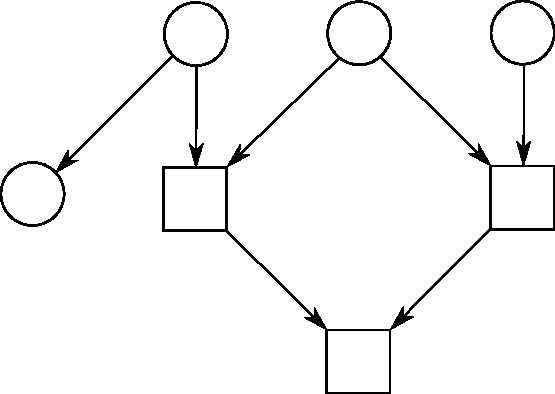
\includegraphics[width=\unitlength]{baysianmodel.pdf}}%
    \put(0.62968498,0.04171382){\color[rgb]{0,0,0}\makebox(0,0)[lb]{\smash{$S$}}}%
    \put(0.33638551,0.33553136){\color[rgb]{0,0,0}\makebox(0,0)[lb]{\smash{$F$}}}%
    \put(0.92239445,0.33553136){\color[rgb]{0,0,0}\makebox(0,0)[lb]{\smash{$C$}}}%
    \put(0.33586739,0.63038521){\color[rgb]{0,0,0}\makebox(0,0)[lb]{\smash{$X$}}}%
    \put(0.62968498,0.63149328){\color[rgb]{0,0,0}\makebox(0,0)[lb]{\smash{$U$}}}%
    \put(0.92671889,0.62934899){\color[rgb]{0,0,0}\makebox(0,0)[lb]{\smash{$T$}}}%
    \put(0.0420857,0.34096392){\color[rgb]{0,0,0}\makebox(0,0)[lb]{\smash{$Z$}}}%
  \end{picture}%
\endgroup%

\resizebox{0.5\textwidth}{!}{%% Creator: Inkscape inkscape 0.48.4, www.inkscape.org
%% PDF/EPS/PS + LaTeX output extension by Johan Engelen, 2010
%% Accompanies image file 'baysianmodel_box_model.pdf' (pdf, eps, ps)
%%
%% To include the image in your LaTeX document, write
%%   \input{<filename>.pdf_tex}
%%  instead of
%%   \includegraphics{<filename>.pdf}
%% To scale the image, write
%%   \def\svgwidth{<desired width>}
%%   \input{<filename>.pdf_tex}
%%  instead of
%%   \includegraphics[width=<desired width>]{<filename>.pdf}
%%
%% Images with a different path to the parent latex file can
%% be accessed with the `import' package (which may need to be
%% installed) using
%%   \usepackage{import}
%% in the preamble, and then including the image with
%%   \import{<path to file>}{<filename>.pdf_tex}
%% Alternatively, one can specify
%%   \graphicspath{{<path to file>/}}
%% 
%% For more information, please see info/svg-inkscape on CTAN:
%%   http://tug.ctan.org/tex-archive/info/svg-inkscape
%%
\begingroup%
  \makeatletter%
  \providecommand\color[2][]{%
    \errmessage{(Inkscape) Color is used for the text in Inkscape, but the package 'color.sty' is not loaded}%
    \renewcommand\color[2][]{}%
  }%
  \providecommand\transparent[1]{%
    \errmessage{(Inkscape) Transparency is used (non-zero) for the text in Inkscape, but the package 'transparent.sty' is not loaded}%
    \renewcommand\transparent[1]{}%
  }%
  \providecommand\rotatebox[2]{#2}%
  \ifx\svgwidth\undefined%
    \setlength{\unitlength}{286.6095bp}%
    \ifx\svgscale\undefined%
      \relax%
    \else%
      \setlength{\unitlength}{\unitlength * \real{\svgscale}}%
    \fi%
  \else%
    \setlength{\unitlength}{\svgwidth}%
  \fi%
  \global\let\svgwidth\undefined%
  \global\let\svgscale\undefined%
  \makeatother%
  \begin{picture}(1,0.78509323)%
    \put(0,0){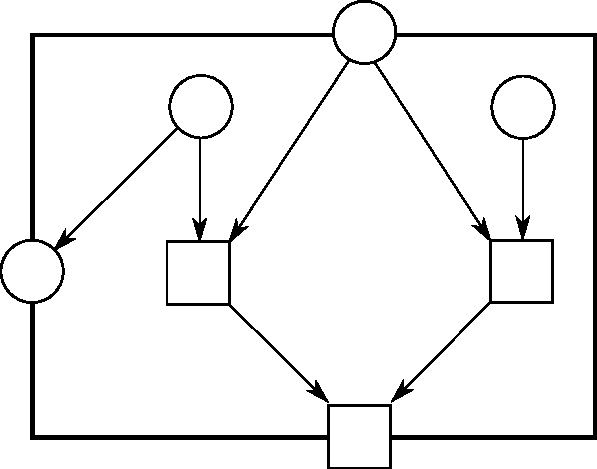
\includegraphics[width=\unitlength]{baysianmodel_box_model.pdf}}%
    \put(0.31103133,0.31530351){\color[rgb]{0,0,0}\makebox(0,0)[lb]{\smash{$F_i$}}}%
    \put(0.85906585,0.31822343){\color[rgb]{0,0,0}\makebox(0,0)[lb]{\smash{$C_i$}}}%
    \put(0.3207583,0.59357303){\color[rgb]{0,0,0}\makebox(0,0)[lb]{\smash{$X_i$}}}%
    \put(0.86459435,0.59265798){\color[rgb]{0,0,0}\makebox(0,0)[lb]{\smash{$T_i$}}}%
    \put(0.03874787,0.31903892){\color[rgb]{0,0,0}\makebox(0,0)[lb]{\smash{$Z_i$}}}%
    \put(0.58873498,0.71586238){\color[rgb]{0,0,0}\makebox(0,0)[lb]{\smash{$U_i$}}}%
    \put(0.59076283,0.03856025){\color[rgb]{0,0,0}\makebox(0,0)[lb]{\smash{$S_i$}}}%
  \end{picture}%
\endgroup%
}
\captionsetup{justification=raggedright}
\caption{Encapsulation of the original graphical model.}
\label{fig:boxmodel}
\end{figure}	
\begin{figure}[!htbp]
\centering
%\def\svgwidth{0.6\linewidth} 
%%% Creator: Inkscape inkscape 0.48.4, www.inkscape.org
%% PDF/EPS/PS + LaTeX output extension by Johan Engelen, 2010
%% Accompanies image file 'baysianmodel.pdf' (pdf, eps, ps)
%%
%% To include the image in your LaTeX document, write
%%   \input{<filename>.pdf_tex}
%%  instead of
%%   \includegraphics{<filename>.pdf}
%% To scale the image, write
%%   \def\svgwidth{<desired width>}
%%   \input{<filename>.pdf_tex}
%%  instead of
%%   \includegraphics[width=<desired width>]{<filename>.pdf}
%%
%% Images with a different path to the parent latex file can
%% be accessed with the `import' package (which may need to be
%% installed) using
%%   \usepackage{import}
%% in the preamble, and then including the image with
%%   \import{<path to file>}{<filename>.pdf_tex}
%% Alternatively, one can specify
%%   \graphicspath{{<path to file>/}}
%% 
%% For more information, please see info/svg-inkscape on CTAN:
%%   http://tug.ctan.org/tex-archive/info/svg-inkscape
%%
\begingroup%
  \makeatletter%
  \providecommand\color[2][]{%
    \errmessage{(Inkscape) Color is used for the text in Inkscape, but the package 'color.sty' is not loaded}%
    \renewcommand\color[2][]{}%
  }%
  \providecommand\transparent[1]{%
    \errmessage{(Inkscape) Transparency is used (non-zero) for the text in Inkscape, but the package 'transparent.sty' is not loaded}%
    \renewcommand\transparent[1]{}%
  }%
  \providecommand\rotatebox[2]{#2}%
  \ifx\svgwidth\undefined%
    \setlength{\unitlength}{266.48922058bp}%
    \ifx\svgscale\undefined%
      \relax%
    \else%
      \setlength{\unitlength}{\unitlength * \real{\svgscale}}%
    \fi%
  \else%
    \setlength{\unitlength}{\svgwidth}%
  \fi%
  \global\let\svgwidth\undefined%
  \global\let\svgscale\undefined%
  \makeatother%
  \begin{picture}(1,0.7093861)%
    \put(0,0){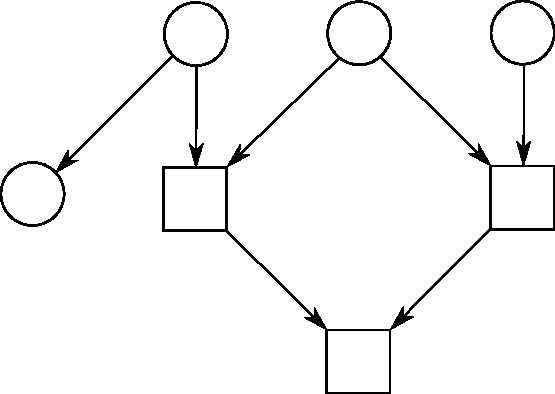
\includegraphics[width=\unitlength]{baysianmodel.pdf}}%
    \put(0.62968498,0.04171382){\color[rgb]{0,0,0}\makebox(0,0)[lb]{\smash{$S$}}}%
    \put(0.33638551,0.33553136){\color[rgb]{0,0,0}\makebox(0,0)[lb]{\smash{$F$}}}%
    \put(0.92239445,0.33553136){\color[rgb]{0,0,0}\makebox(0,0)[lb]{\smash{$C$}}}%
    \put(0.33586739,0.63038521){\color[rgb]{0,0,0}\makebox(0,0)[lb]{\smash{$X$}}}%
    \put(0.62968498,0.63149328){\color[rgb]{0,0,0}\makebox(0,0)[lb]{\smash{$U$}}}%
    \put(0.92671889,0.62934899){\color[rgb]{0,0,0}\makebox(0,0)[lb]{\smash{$T$}}}%
    \put(0.0420857,0.34096392){\color[rgb]{0,0,0}\makebox(0,0)[lb]{\smash{$Z$}}}%
  \end{picture}%
\endgroup%

\resizebox{1\textwidth}{!}{%% Creator: Inkscape inkscape 0.48.4, www.inkscape.org
%% PDF/EPS/PS + LaTeX output extension by Johan Engelen, 2010
%% Accompanies image file 'graphicalModel_temporal.pdf' (pdf, eps, ps)
%%
%% To include the image in your LaTeX document, write
%%   \input{<filename>.pdf_tex}
%%  instead of
%%   \includegraphics{<filename>.pdf}
%% To scale the image, write
%%   \def\svgwidth{<desired width>}
%%   \input{<filename>.pdf_tex}
%%  instead of
%%   \includegraphics[width=<desired width>]{<filename>.pdf}
%%
%% Images with a different path to the parent latex file can
%% be accessed with the `import' package (which may need to be
%% installed) using
%%   \usepackage{import}
%% in the preamble, and then including the image with
%%   \import{<path to file>}{<filename>.pdf_tex}
%% Alternatively, one can specify
%%   \graphicspath{{<path to file>/}}
%% 
%% For more information, please see info/svg-inkscape on CTAN:
%%   http://tug.ctan.org/tex-archive/info/svg-inkscape
%%
\begingroup%
  \makeatletter%
  \providecommand\color[2][]{%
    \errmessage{(Inkscape) Color is used for the text in Inkscape, but the package 'color.sty' is not loaded}%
    \renewcommand\color[2][]{}%
  }%
  \providecommand\transparent[1]{%
    \errmessage{(Inkscape) Transparency is used (non-zero) for the text in Inkscape, but the package 'transparent.sty' is not loaded}%
    \renewcommand\transparent[1]{}%
  }%
  \providecommand\rotatebox[2]{#2}%
  \ifx\svgwidth\undefined%
    \setlength{\unitlength}{514.815004bp}%
    \ifx\svgscale\undefined%
      \relax%
    \else%
      \setlength{\unitlength}{\unitlength * \real{\svgscale}}%
    \fi%
  \else%
    \setlength{\unitlength}{\svgwidth}%
  \fi%
  \global\let\svgwidth\undefined%
  \global\let\svgscale\undefined%
  \makeatother%
  \begin{picture}(1,0.36762093)%
    \put(0,0){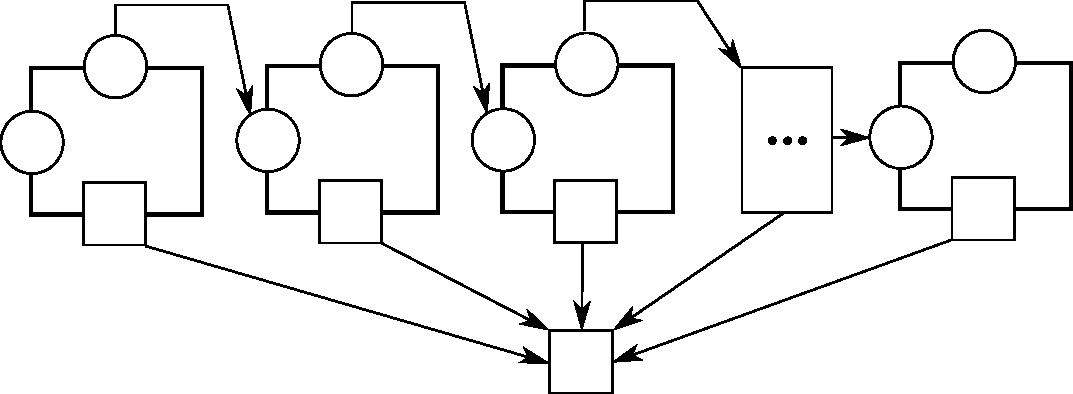
\includegraphics[width=\unitlength]{graphicalModel_temporal.pdf}}%
    \put(0.09547193,0.29665535){\color[rgb]{0,0,0}\makebox(0,0)[lb]{\smash{$U_0$}}}%
    \put(0.09407952,0.15956687){\color[rgb]{0,0,0}\makebox(0,0)[lb]{\smash{$S_0$}}}%
    \put(0.01881458,0.22563278){\color[rgb]{0,0,0}\makebox(0,0)[lb]{\smash{$Z_0$}}}%
    \put(0.31237857,0.29852096){\color[rgb]{0,0,0}\makebox(0,0)[lb]{\smash{$U_1$}}}%
    \put(0.31409408,0.16143247){\color[rgb]{0,0,0}\makebox(0,0)[lb]{\smash{$S_1$}}}%
    \put(0.23882916,0.22749837){\color[rgb]{0,0,0}\makebox(0,0)[lb]{\smash{$Z_1$}}}%
    \put(0.90558919,0.30139354){\color[rgb]{0,0,0}\makebox(0,0)[lb]{\smash{$U_n$}}}%
    \put(0.90419676,0.16430507){\color[rgb]{0,0,0}\makebox(0,0)[lb]{\smash{$S_n$}}}%
    \put(0.82893184,0.23037096){\color[rgb]{0,0,0}\makebox(0,0)[lb]{\smash{$Z_n$}}}%
    \put(0.53050271,0.02213156){\color[rgb]{0,0,0}\makebox(0,0)[lb]{\smash{$S_f$}}}%
    \put(0.53175169,0.29895161){\color[rgb]{0,0,0}\makebox(0,0)[lb]{\smash{$U_2$}}}%
    \put(0.53346717,0.16186314){\color[rgb]{0,0,0}\makebox(0,0)[lb]{\smash{$S_2$}}}%
    \put(0.4582022,0.22792902){\color[rgb]{0,0,0}\makebox(0,0)[lb]{\smash{$Z_2$}}}%
  \end{picture}%
\endgroup%
}
\captionsetup{justification=raggedright}
\caption{Chaining of the original graphical models.}
\label{fig:dbnet}
\end{figure}	
To describe the problem using a graphical model, we need to extend the above model in a temporal fashion. In Fig.~\ref{fig:boxmodel}, we first encapsulate the original graphical model into a block, where three variables are exposed to the outside. Then we chain the small blocks in series to obtain a new model as depicted in Fig.~\ref{fig:dbnet}. We use subscript $0,1,\cdots i$ to indicate the time dependency of the variables. The grasp process begins with the first measurement in time stamp zero. As a result, a dependency is created between $X_0$ and $Z_0$. Based on the sensing result, a control trajectory $U_0 = u_0$ is inferred to maximize the probability of success $S_0$. The robot performs one step of the trajectory $u_0$ and the grasping process moves on to the next time stamp. Since the camera also moves towards the object, the measurement at the next time stamp $Z_1$ depends on the last trajectory $U_0$ and the object state $X_1$. The sensing and control loop repeats until the last measurement $Z_i$ and control trajectory $U_i$ are taken. The conditional probability of success is formulated by 
\begin{equation}
 \pr(S_f=1| \underline{Z} = \underline{z},  \underline{U} = \underline{u}, \underline{T} = \underline{t}) = \frac{\sum\limits_{\substack{F_0,\cdots,F_n,\\ C_0,\cdots,C_n \\ X_0,\cdots X_n \\ S_0,\cdots S_n} }\pr( S = 1, \underline{F}, \underline{C}, \underline{X}, \underline{z},\underline{u}, \underline{t})} {P(\underline{Z} = \underline{z},  \underline{U} = \underline{u}, \underline{T} = \underline{t})} 
\label{equ:condition_prob_limit_sensing} 
\end{equation}
where $\underline{Z} = \{Z_0, \cdots, Z_n\}$, $ \underline{U} = \{U_0, \cdots, U_n\}$ and $\underline{C} = \{C_0, \cdots, C_n\}$. The condition $\underline{t} = \{t, \cdots, t\}$ indicates in each time stamp the task specifications are the same. Again, the nominator is computed by marginalizing the joint probability of all the variables  which are neither query nor conditions. The denominator is a renormalization constant. The joint probability distribution in the nominator can be computed based on the graph structure by 
\begin{equation}
\begin{split}
\pr( S_f = 1, \underline{F}, \underline{C}, \underline{X}, \underline{z},\underline{u},\underline{t}) = \prod\limits_{i = 1:n} &\pr(F_i | X_i, u_i) \cdot \pr(C_i | u_i, t)\cdot   \pr(z_i|u_{i-1}, X_i) \\
              \cdot & \pr(F_0 | X_0, u_0)\cdot \pr(C_0 | u_0, t)  \pr(z_0|X_0 )\\
              \cdot &\pr(S_i | F_i, C_i) \cdot  \pr(S_f=1| S_1, \cdots, S_n)   \\
              \cdot &\pr(X_i)\cdot P(u_i) \cdot\pr(X_0) \cdot \pr(u_0) 
\end{split}
\label{equ:cpd_graph}
\end{equation}
First, we eliminate discrete variables $\underline{F}$, $\underline{C}$ and $\underline{S}$.
The term $\pr(S_f=1| S_1, \cdots, S_n)$ equals zero as long as one of the $S_i$ does not equal to one. Therefore, after marginalization of $\underline{S}$ the nominator equals
\begin{equation}
\begin{split}
\sum\limits_{\substack{F_0,\cdots,F_n,\\ C_0,\cdots,C_n \\ X_0,\cdots X_n \\ S_0,\cdots S_n} }\pr( S_f = 1, \underline{F}, \underline{C}, \underline{X}, \underline{z},\underline{u}, \underline{t}) = \sum\limits_{\substack{F_0,\cdots,F_n,\\ C_0,\cdots,C_n \\ X_0,\cdots X_n  }} \pr( S_f = 1, \underline{S} = \underline{1}, \underline{F}, \underline{C}, \underline{X}, \underline{z},\underline{u}, \underline{t})
\end{split}
\label{equ:after_maginalizing_s}
\end{equation}
The same principle also applies to $F_i$ and $C_i$, because the term $\pr(S_i = 1 | F_i, C_i)$ equals zero everywhere except at $F_i=1,C_i=1 $. After we eliminate all the  $F_i$ and $C_i$, the nominator of equation \ref{equ:condition_prob_limit_sensing} equals to 
\begin{equation}
\begin{split}
\sum\limits_{\substack{F_0,\cdots,F_n,\\ C_0,\cdots,C_n \\ X_0,\cdots X_n \\ S_0,\cdots S_n} }\pr( S_f = 1, \underline{F}, \underline{C}, \underline{X}, \underline{z},\underline{u}, \underline{t}) = \sum\limits_{ X_0,\cdots X_n } \pr( S_f = 1, \underline{S} = \underline{1}, \underline{F} = \underline{1}, \underline{C} = \underline{1}, \underline{X}, \underline{z},\underline{u}, \underline{t})
\end{split}
\label{equ:after_maginalizing_cf}
\end{equation}
Substituting the term after sum operation by \ref{equ:cpd_graph}, we obtain 
\begin{equation}
\begin{split}
 &\sum\limits_{ X_0,\cdots X_n } \pr( S_f = 1, \underline{S} = \underline{1}, \underline{F} = \underline{1}, \underline{C} = \underline{1}, \underline{X}, \underline{z},\underline{u}, \underline{t}) \\
=&\sum\limits_{ X_0,\cdots X_n } \prod\limits_{i = 1:n} \pr(F_i=1 | X_i, u_i) \cdot \pr(C_i = 1 | u_i, t)\cdot   \pr(z_i|u_{i-1}, X_i) \\
              \cdot & \pr(F_0=1 | X_0, u_0)\cdot \pr(C_0=1 | u_0, t)  \pr(z_0|X_0 )\\
              \cdot & \underbrace{\pr(S_i = 1 | F_i = 1, C_i=1)}_{=1} \cdot  \underbrace{\pr(S_f=1| S_1, \cdots, S_n = 1)}_{=1}  \\
              \cdot &\pr(X_i)\cdot P(u_i) \cdot\pr(X_0) \cdot \pr(u_0) \\
=&  \prod\limits_{i = 1:n} \underbrace{   \sum\limits_{ X_i} \pr(F_i=1 | X_i, u_i) \cdot \pr(C_i = 1 | u_i, t)\cdot   \pr(z_i|u_{i-1}, X_i) \cdot \pr(X_i) }_{\phi_i(u_i, u_{i-1}) } \\ 
  & \cdot \underbrace{ \sum\limits_{ X_0} \pr(F_0 =1 | X_0, u_0)\cdot \pr(C_0=1 | u_0, t)  \pr(z_0|X_0 ) \cdot \pr(X_0) }_{\phi_0(u_0)} \\ 
  &  \cdot \underbrace{ \pr(u_i) \cdot \pr(u_0) }_{\text{constant}} \\
  \propto &  \prod\limits_{i = 1:n} \phi_i(u_i, u_{i-1}) \cdot \phi_0(u_0).
\end{split}
\end{equation}

Incorporating the renormalization constant in the denominator of Equ.~\ref{equ:condition_prob_limit_sensing}, the conditional probability of grasping success is proportional to the multiplication of a set of factors $\phi_i$.    
\begin{equation}
\begin{split}
&  \pr(S_f=1| \underline{Z} = \underline{z},  \underline{U} = \underline{u}, \underline{T} = \underline{t}) \\
\propto & \prod\limits_{i = 1:n} \phi_i(u_i, u_{i-1}) \cdot \phi_0(u_0).
\end{split}
\end{equation}
As same as in the previous grasping scenario, we aim to find $u_0^*$ to $u_n^*$ to maximize the conditional probability. However, due to the temporal property of the model, we can not condition all the measurements $\underline{Z}$ at once. The conditioning of the measurement depends on what control trajectory $u$ is sent to the robot at the last time stamp. Therefore, the optimal control sequence  $u_0^*:u_t^*$ can only be found in an iterative fashion. We propose to use the following paradigm to find optimal controls for the robot. 
\begin{algorithm}[!htbp]
\begin{algorithmic}[1]
\STATE $u_0^*  = \argmax\limits_{u_0}  \phi_0(u_0)   $
\STATE execute $u_0^*$ on robot 
\STATE wait for a time step
\FOR {$i$ from 1 to $n$}
\STATE $u_i^*  = \argmax\limits_{u_i}  \phi_i(u_i ,u_{i-1}^* ) $ 
\STATE execute $u_i^*$ on robot 
\STATE wait for a time step 
\IF {pre-touch configuration is reached}
\RETURN success
\ENDIF
\ENDFOR 
%\captionsetup{justification=raggedright}
\caption {Paradigm for iteratively finding optimal control trajectory}
\label{paradigmforgrasping}
\end{algorithmic}
\end{algorithm}

 \section{Summary}
 In this chapter, we first propose a unified model based on Bayesian networks to describe grasping problems. The network we define for the grasping problem factorizes the joint distribution into smaller conditional probability distributions. By conditioning on a subset of variables such as measurement and robot controls, we can compute the conditional probability of success. The goal is to determine the controls that maximize the conditional probability of success. Then we derive how to compute the conditional success probability in three different grasping scenarios. The focus of each scenario is different. In the first scenario, we consider grasping known objects under task constraint. As the object is known to the robot, force closure and representation of the object are not an issue. The focus in this scenario is how to model the task constraint satisfaction. In the second scenario, we consider the problem of grasping unknown objects. The focus is how to model the probability of force closure and how to model the object. In the third scenario, we consider the problem that the robot only has limited sensing capability. To reduce perception uncertainty, the model is extended in a temporal fashion to allow continuous measurement integration. The focus is how to find optimal controls online in each iteration. In the following chapters, we will elaborate how the grasping problem is solved in each grasping scenarios.




 
